\section{AD Wandler \hartl{475}}

\subsection{Parallelverfahren und Kaskadenumsetzer}
\begin{longtable}{|p{12cm}|c|}
\hline
  {\textbf{Parallelumsetzer} \hartl{478}
  \begin{itemize}
    \item sehr schnell
    \item $2^n$ Widerstände
    \item $2^N$ Komparatoren
  \end{itemize}
  \begin{align*}
    Anz_{Vergleiche}=2^N-1
  \end{align*}}
  &
  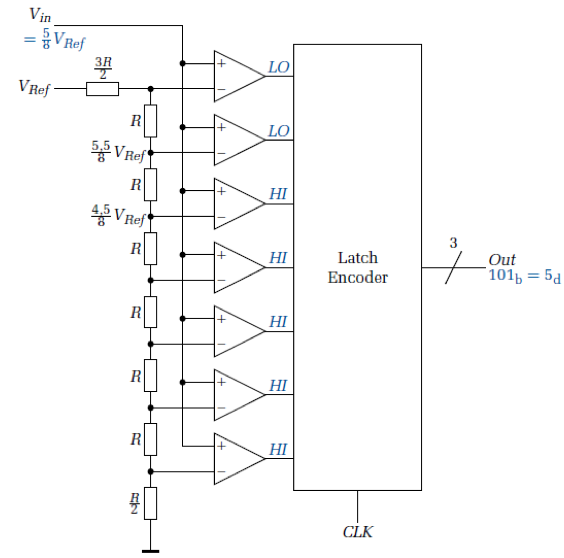
\includegraphics[width=6cm, valign=t]{pictures/parallelADC}\\ 
\hline

  {\textbf{Kaskadenumsetzer}\hartl{479}\newline 
  Eine 10-bit-Auflösung beim Parallelverfahren würde 1024 Komperatoren
  benötigen.$\Rightarrow$Komplexitätsreduktion \newline
  Mit erstem $N_{1}$-bit ADU wird der Grobbereich festgelegt (höherwertige
  Bits).
  Diese Zahl wird in eine analoge Spannung durch einen $N_{1}$-bit DAU zurück
  umgesetzt und diese Spannung von der Eingangsspannung subtrahiert. Diese
  Differenz wird von einem weiteren $N_{1}$-bit-ADU umgesetzt, um die
  niederwertigen Bits zu ergeben. Skaliert man die Differenzspannung mit dem
  Faktor 32, hat man den gleichen Spannungsbereich, kann also zwei identische
  ADC benutzen.
  }
  &
  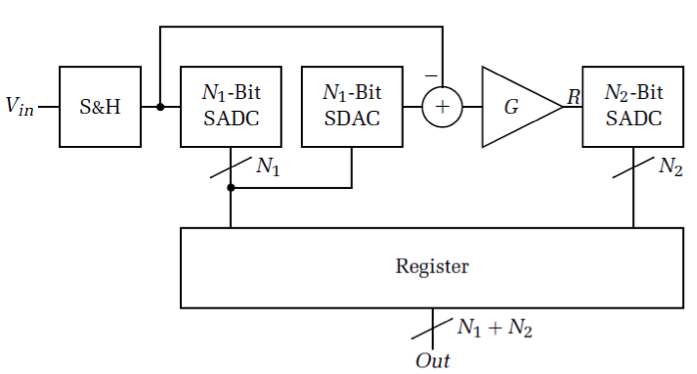
\includegraphics[width=6cm, valign=t]{pictures/kaskaden}\\ 
\hline

  {\textbf{Pipelined ADC} \hartl{483}
  \begin{itemize}
    \item fast gleiche hohe Umsetzrate wie Parallelumsetzer
    \item gleicher schaltungstechnischer Aufwand wie beim Kaskadennumsetzer
    \item wird heute für schnelle ADC's verwendet
  \end{itemize}
  }
  &
  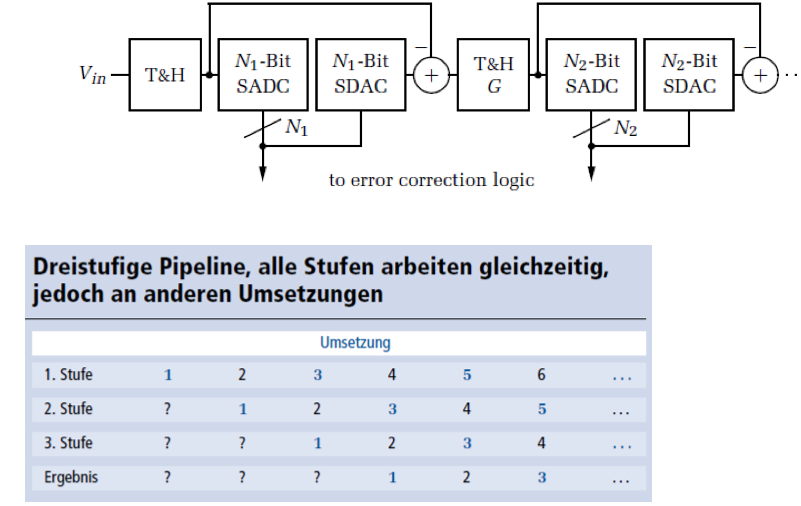
\includegraphics[width=6cm, valign=t]{pictures/pipelined}\\ 
\hline
\end{longtable}

\subsection{Wägeverfahren ( sukzessive Approximation) \hartl{485}}
\begin{longtable}{|p{12cm}|c|}
\hline
  \multirow{2}{12cm}{\textbf{Prinzip} \hartl{485}
  \begin{itemize}
    \item Abtastung der Eingangsspannung $V_{in}$mit einer
        S\&H-Schaltung( Vergleichsspannung liegt so während der gesamten
      Umsetzung an)
    \item Vergleich starte in der Mitte der Eingangsspannung $\frac{V_{Ref}}{2}$
    \item Tabelle mit Beispiel: \hartl{487}
  \end{itemize}
  }
  &
  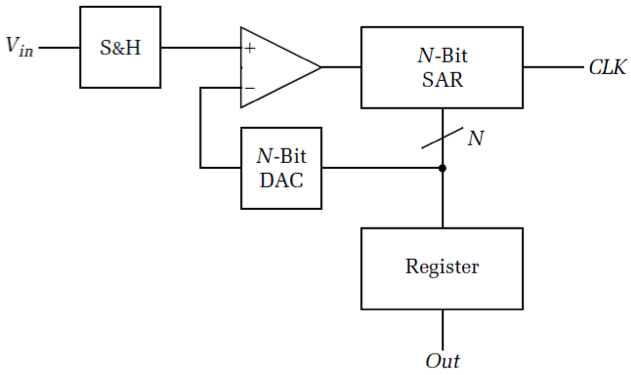
\includegraphics[width=6cm, valign=t]{pictures/waegeverfahren}
  \\ \hline
  \textbf{Wägeverfahren mit SC-Prinzip} \hartl{488} \newline
  { \begin{align*}
  	b &= 3 & \text{Quantisierung} \\
  	q &= \frac{V_{ref}}{2^b} & \text{Quantisierungsschritt} \\
  	D &= floor\left(\frac{V_{in}}{q}\right) & \text{Digitaler Wert} \\
  	V_{rest} &= mod\left(V_{in},q\right) & \text{nicht aufgelöste Spannung}
  \end{align*}}
  &
  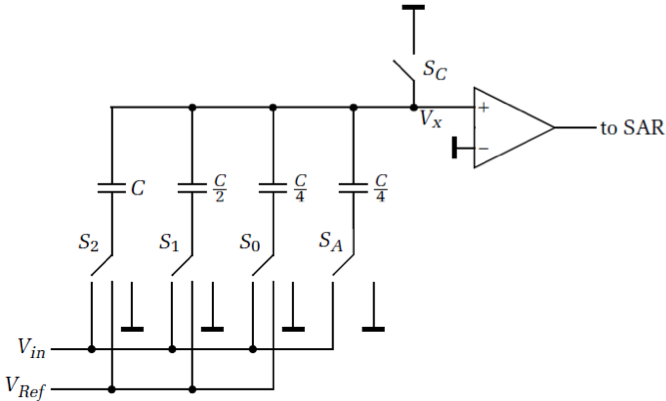
\includegraphics[width=6cm, valign=t]{pictures/waegeverfahrenSC}\\
\hline

  {\textbf{Iterative ADC}
  \begin{enumerate}
    \item Im S/H wird die Eingangsspannung geschpeichert (Schalter Sin)
    \item Schalter Sin wird danach auf den Multiplizierer-Ausgang geschaltet
    \item X(Laufvariable) wird auf n-1 gesetzt
    \item Der Komparator wird ausgewertet\newline
      Dout=1: Bx=1, Switch S=1 (d.h. im Subtrahierer wird Vrefh von Vc
      subtrahiert)\newline
      Dout=0: Bx=0, Switch S=0 (d.h. im Subtrahierer wird 0 von Vc
      subtrahiert)
    \item Der Subtrahierer generiert sein Ausgangssignal
    \item Der Multiplizierer generiert sein Ausgangssignal
    \item Im S/H wird die Feedback-Spannung gespeichert (Schalter Sin)
    \item X wird um 1 reduziert
    \item Gehe zu Schritt 4, wenn $X\geq0$
  \end{enumerate}
  }
  &
  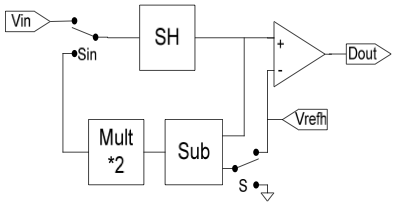
\includegraphics[width=6cm, valign=t]{pictures/iterativeADC}\\
\hline
\end{longtable}



\subsection{Zählverfahren \hartl{490}} 
Ist für kontinuierliche Auswertungen des Eingangssignal
\subsubsection{Single Slope}

\begin{tabular}{ccp{4cm}}
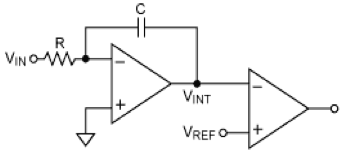
\includegraphics[width=6cm, valign=t]{pictures/singleSlope1}
&
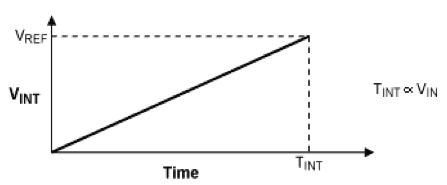
\includegraphics[width=6cm, valign=t]{pictures/singleSlope2}
&
  {\begin{align*}
    T_{int}=\frac{V_{Ref} \cdot R \cdot C}{V_{in}}
  \end{align*}}
\\ 
\end{tabular}

\subsubsection{Dual Slope \hartl{492}}
\begin{longtable}{cp{12cm}}
 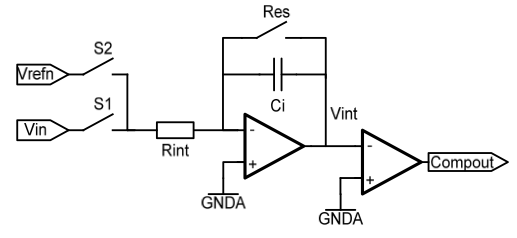
\includegraphics[width=6cm, valign=t]{pictures/dualSlope11}
 & 
 \textbf{Für $0<t<T_{int}$}
 \vspace{0.2cm}
 {\begin{align*}
      V(t)&=
      \int\limits_0^{t}\frac{-1}{R_{int}
      \cdot C_{i}}(V_{in}-V_{GNDA})d\tau+V_{GNDA}\\
      V_{int}(V_{in})&=\frac{-1}{R_{int}
      \cdot C_{i}}(V_{in}-V_{GNDA})T_{int}+V_{GNDA}\\
      V_{intmax}&=V_{int}(V_{in}=0)\\
                &=\frac{-1}{R_{int}
      \cdot C_{i}}(-V_{GNDA})T_{int}+V_{GNDA}
 \end{align*}} \\
 
 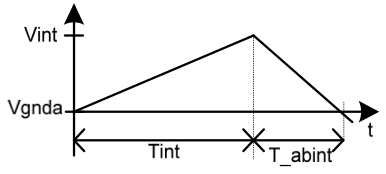
\includegraphics[width=6cm, valign=t]{pictures/dualSlope12}
 &  
 \textbf{Für $T_{int}<t<T$}
 \vspace{0.2cm}
 {\begin{align*}
  V(t)&=V_{int}-\frac{1}{R_{int}\cdot C_{i}}\cdot
  (V_{refn}-V_{GNDA}) \cdot t\\
   T_{abint}&=\frac{(V_{GNDA}-V_{in}) \cdot T_{int}}{V_{refn}-V_{GNDA}}
 \end{align*}}\\
 
 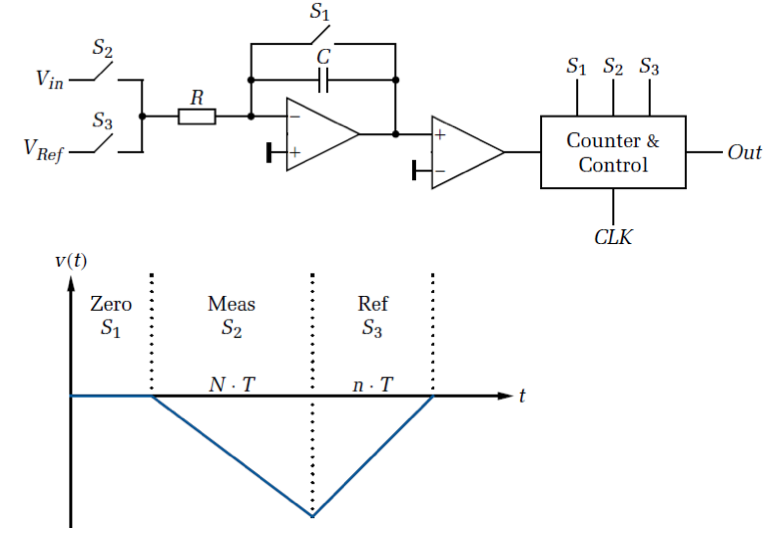
\includegraphics[width=6cm, valign=t]{pictures/dualSlope2}
 &  
 \textbf{Für $V_{GNDA}=0$}
 \vspace{0.2cm}
 {\begin{align*}
    \int^{N\cdot T}_{0}V_{in}dt&=N \cdot T \cdot V_{in}\\
      N \cdot T \cdot V_{in}-\int^{n \cdot T}_{0}V_{Ref}dt&=N \cdot T \cdot V_{in}-n \cdot T \cdot V_{Ref}=0\\
      n&=\frac{V_{in}}{V_{Ref}}N\\
  \end{align*}}\\
  
  
  \begin{tabular}{ll}
      N:&Taktzyklen\\
      T:&Periodendauer\\
      n:&Zählerstand\\
      $V_{off}$:&Offsetspannung\\
  \end{tabular}
  &
  
  \begin{tabular}{ll}
      $T_{int}$:&Integrationszeit\\
      $T_{abint}$:& "`Messzeit"\\
      $V_{int}$:&Spannung am $V_{opOut}$ nach der Zeit $T_{int}$\\
      $V_{intmax}:$&maximal mögliche Spannung am $V_{opOut}$\\
  \end{tabular}
\end{longtable}

\subsubsection{Spannungs- Frequenz- Umsetzer \hartl{495}}
\begin{multicols}{2}
\setlength{\columnseprule}{1pt}
	\begin{center}
  		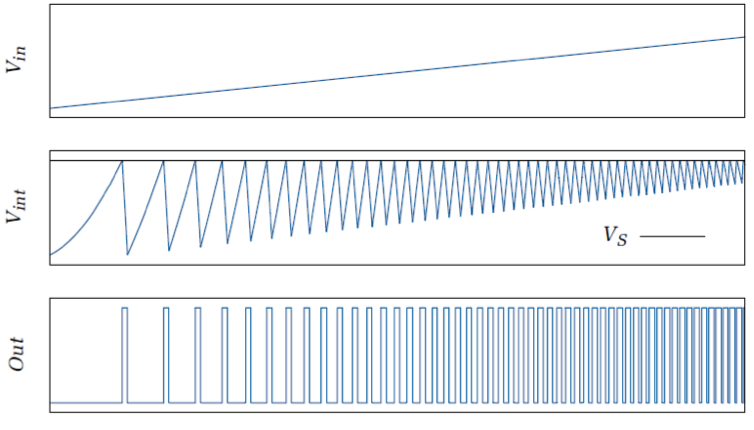
\includegraphics[width=7cm]{pictures/sfu_kurven}
  	\end{center}
  
  
  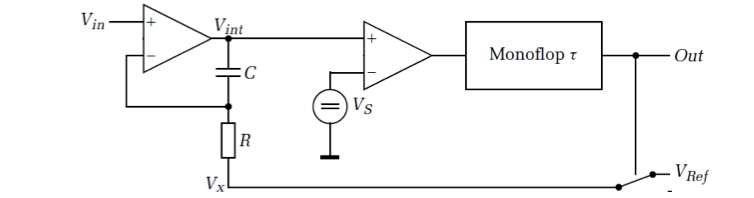
\includegraphics[width=6cm]{pictures/sfu_schaltung}
  
   \begin{align*}
      V_{int}(t)=V_{in}+\frac{1}{RC}\int(V_{in}-V_{x})dt
   \end{align*}
    Vorteil: Immer am Eingangssignal\newline
    Nachteil: Kein echter ADC  


\subsubsection{Ladungs-Ausgleichs-Integrator \hartl{497}}
	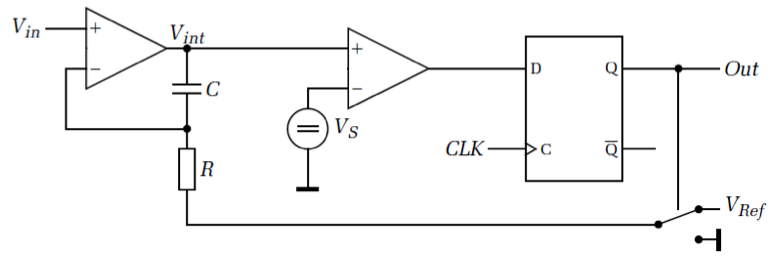
\includegraphics[width=6cm, valign=t]{pictures/lsg1} \\
	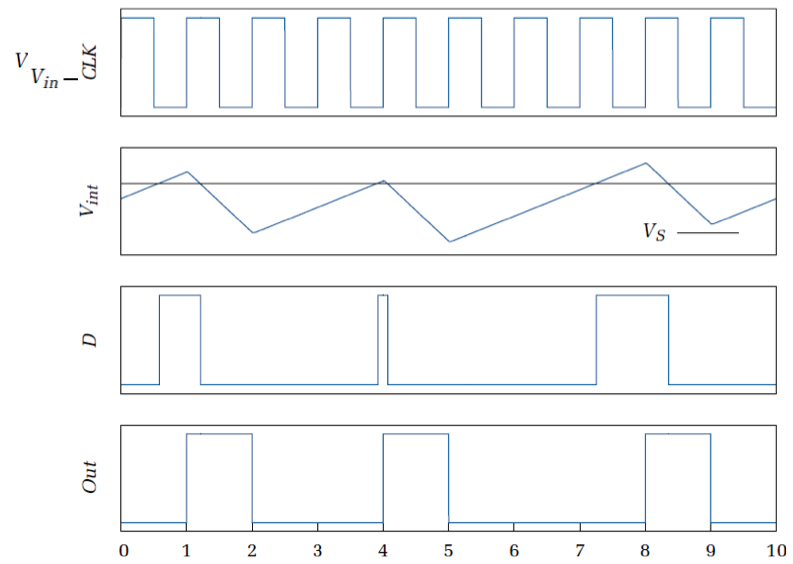
\includegraphics[width=6cm, valign=t]{pictures/lsg2}
	\begin{itemize}
	   \item Gleichgewichtsbedingung\\
	    \begin{equation*}
	      V_{in}-\frac{n}{N}V_{Ref}=0\Rightarrow n=\frac{V_{in}}{V_{Ref}}N
	    \end{equation*}
	  \item Flipflop statt Monoflop
	\end{itemize}
	
	
\subsubsection{Sigma-Delta Wandler \hartl{500}}
	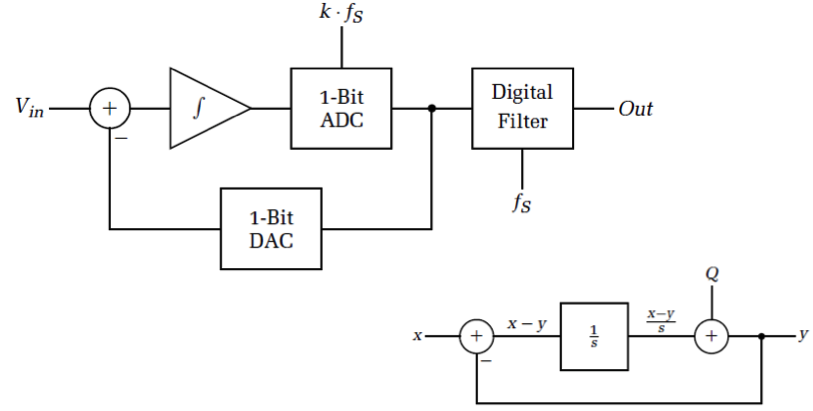
\includegraphics[width=6cm, valign=t]{pictures/deltaSigma1}
	\begin{itemize}
	      \item Ersatzschaltung für Frequenzbereich
	      \item Tiefpass für Signal
	      \item Hochpass für Q
	\end{itemize}
	\begin{align*}
	  y=\frac{x-y}{s}+Q\Rightarrow y=x\frac{1}{1+s}+Q\frac{s}{1+s}
	\end{align*}


\subsubsection{Sigma-Delta Wandler 2. Ordnung \hartl{502}}
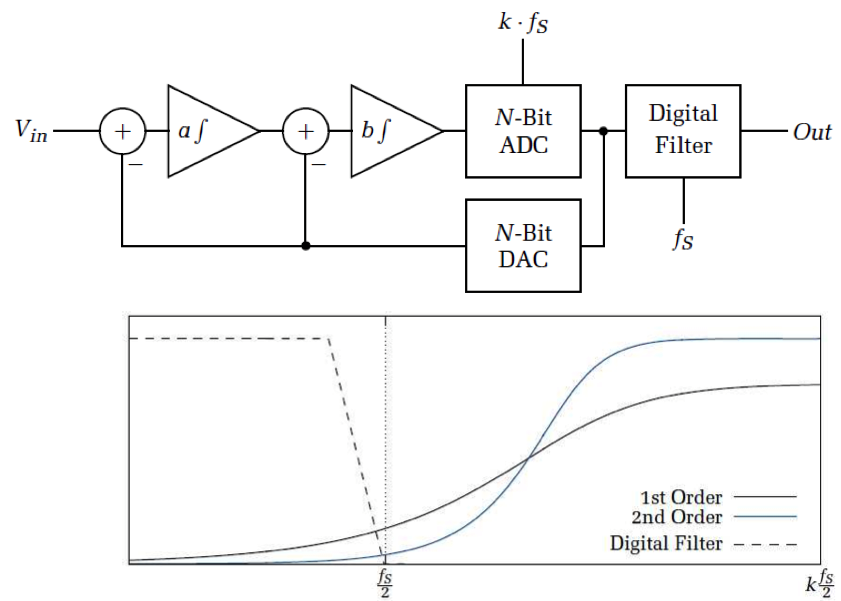
\includegraphics[width=6cm, height =4cm]{pictures/deltaSigma2}


\subsection{Kennwerte von ADC's}
Siehe Buch \hartl{505}!

\end{multicols}
